\documentclass[english]{article}\usepackage[]{graphicx}\usepackage[]{color}
\usepackage{alltt}
\usepackage[T1]{fontenc}
\usepackage[latin9]{inputenc}
\usepackage{geometry}
\geometry{verbose}
\setcounter{secnumdepth}{2}
\setcounter{tocdepth}{2}
\usepackage{amsmath}
\usepackage{graphicx}
\usepackage{esint}
\usepackage{algpseudocode}
\usepackage{algorithm}
\usepackage{babel}
\usepackage{verbatim} % for \begin{comment}
\usepackage{subcaption}
\usepackage{float}
\IfFileExists{upquote.sty}{\usepackage{upquote}}{}
\begin{document}

\title{Autonomous Robots and Environmental Mapping}

\author{M. Horning, M. Lin, S. Srinivasan, S. Zou}

\maketitle

\begin{abstract}

Compressed sensing is a technique used to reconstruct sparse signals and images while sampling well below the Nyquist rate. Commonly used in fMRIs and medical imaging, we aim to use this technique to allow autonomous robots to map piecewise constant areas of interest within a larger environment. In our experiment, we programmed a robot equipped with a reflectance sensor to travel along straight-line paths on a black testbed with white regions of interest. The robot integrated sensor readings and sent that sum to a remote server after each path. Each data point consists of the robot's start and end positions, tracked by an overhead camera, and the integral found along that path. Once all the data has been collected, the environment is reconstructed by minimizing the sum of the data fitting term and an L1 penalty term. We also implemented an "adaptive path selection scheme", allowing the robot to more intelligently target regions of interest based on the data collected from an initial set of random paths. We have run simulations of adaptive path selection and reconstruction of 100x100 images with only 100 data points gives relative err. = 0.28. We have also carried out experimental trials with the robot and found promising results, but these require further testing.

\end{abstract}

\pagebreak
\tableofcontents
\pagebreak

\section{Introduction}

\begin{comment}
Discuss Compressed Sensing
\end{comment}

Environment mapping is amongst the foundational problems of mobile robotics. In order for an autonomous vehicle to operate effectively within an environment, 

The task of mapping an unknown environment is well-studied in the area of autonomous robotics. 

Compressed sensing describes a technique in which a signal is reconstructed by solving an underdetermined linear system. Doing so allows a signal to be found from a relatively small amount of data. 

%%%%%%%%%%%%%%%%%%%%%%%%%%%%%%%%%%%% LAB SETUP %%%%%%%%%%%%%%%%%%%%%%%%%%%%%%%%%%%%%%%%%%%%%%%%%%%
\section{Lab Setup}
\subsection{Overview}
The setup in the UCLA Applied Mathematics Laboratory (AML) consists of three main components: 

\begin{itemize}
\item A robot vehicle on a black 1.5 m x 2.0 m rectangular test bed made of black asphalt felt paper
\item 2 Overhead Imaging Source DMK 21F04 1/4 Monochrome CCD cameras
\item A Server hosted on a Windows Computer
\end{itemize}

\subsection{Robot}

The robot itself consists of 5 main components:
\begin{enumerate}
\item \textbf{An Arduino Uno with an AdaFruit WiFi Shield:}
		The WiFi Shield allows the Arduino to connect to a network, and so communicate with the server. The WiFi Shield uses up digital pins 3, 4, 5, 10, 11, 12 and 13. Digital Pins 6, 7, 8, 9 connect to the Motor Controller, while analog pin 4 is used to connect to the reflectance sensor. The Arduino is powered by a 9V battery and has limited on-board processing power (16 MHz) and memory (32 KB Flash and 2 KB SRAM). The Arduino is uploaded with the code in \texttt{compressedSensing.ino} (see Appendix).
\item \textbf{Analog Reflectance Sensor:} The reflectance sensor measures the reflectance of the surface, but note that brighter (e.g. white) surfaces register low values while darker (e.g. black)  surfaces register higher values. To make the data more intuitive to understand, the data read is subtracted from the maximum reading (found experimentally) of the sensor, so that black surfaces get stored as lower values while white surfaces are stored as higher values. Currently, the raw data from the sensor is not used but instead thresholded so that any sensor readings above the threshold are read as white and those below are read as black. To extend the project to allow reconstruction of images with varying shades of grey, more thresholds will have to be created so that sensor readings within some range map to some colour between black and white.
\item \textbf{Chassis:} The chassis has four motors, that are powered by 5 AA 1.5V batteries. The chassis also has a switch to connect or disconnect the batteries from the motor.
\item \textbf{Motor controller:} The motor controller acts as the intermediary between the Arduino and motors. The board logic operates at 5V, provided by the Arduino but the AA batteries connect to the motor controller and are actually used to drive the motor. The two motors on the left and the two motors on the right are connected parallel to each other, so the voltage applied to a motor on the front will be the same as the voltage applied to a motor at the back on the same side. This setup provides tank steering for the robot. The motor controller has 4 inputs and 4 outputs. Each input maps to an output that controls the voltage applied to one terminal of the motor. As an example, the robot can be made to move forward by applying a high voltage on both the pins that connect to the positive terminal and a low voltage to both the pins that connect to the negative terminal. It can be made to rotate left by applying high voltage to the positive terminal and low voltage to the negative terminal on the left motors, and applying high voltage to the negative terminal and high voltage to the positive terminal. Note that this in contrast to other types of motor controllers that have two inputs for voltage and two inputs for direction to spin the wheels on either side.

\item \textbf{Tag (Visual ID):} A white rectangular tag with a black-tape border and a black header strip is mounted on the motor controller. It serves as a means for the overhead camera to visually identify the robot. Its distinctive shape and design make it hard to confuse with other shapes that appear on the test bed, and hence serves as unique way to identify the robot's position. Ideally, the center of the tag should be directly over the reflectance sensor -- the video camera should really be tracking the reflectance sensor's as it traverses the test bed collecting data.
\end{enumerate}

\subsection{Video Camera}
The cameras have a resolution of 640x480 pixels and a frame rate of 30 fps and are connected to a PC via
firewire. The computer runs \texttt{vehicle\_tracker.py}, a python script used to track the robots as
they move about the test bed. The script utilizes OpenCV to search for contours and recognize the tag
that is fixed on top of the vehicle, and return the robot's current position and orientation. The
orientation is found from the direction of the vector pointing from the tag's center to the header
strip's center. The script obtains three pieces of information by processing the video: the x-coordinate,
the y-coordinate and the heading and writes this data to a COM port in the form $*\$|x|y|\theta|!\textbackslash$n. The COM port should have a USB-Serial Cable plugged in that is connected to a Wi232 transceiver that transmits this serial data over radio.

\subsection{Server}

The server acts as the intermediary between the robot and video camera. The main script on the server is \texttt{robotServer.cgi}. The Arduino, upon connecting to the network will send a request to this script on the
server with its ``state'' and optionally ``data.'' Note that we do not need an internet connection for this project. Rather, it keeps things simpler if the robot and server are connected to the same priavte network. It is possible to host the server on a network with Internet connection, such as UCLA-MATHNET, but the robot ultimately also needs to be on the same network. If the robot and server need to be on different networks, port forwarding needs to be configured on the network that the server is on so that the Arduino's requests actually get sent to the server. This can be a hassle, so it is advised that the robot and server are on the same private network.

To obtain the robot's location, the server reads data from the serial port. The serial port should be connected to a Wi232 transceiver that receives data broadcast by the other Wi232 transceiver.

\subsection{Putting it all together}

We wish to collect some $m$ data points, where $m << n$, the dimension of the image. Each data point consists of the starting location of the robot, the final location of the robot and the sum of the reflectance sensor values obtained as it travelled in a straight line between the two points. The robot operates as a finite state machine. It consists of binary states, and they function as follows:
\begin{itemize}
\item State 0: When the robot is in state 0, it is either moving/turning to its new start position or requesting the server to confirm it position as it is about to start travelling along a new path and collect data. Note that when the robot is getting into its new start position, there is no communication with the server. This happens everytime the robot switches to state 0 from state 1.
\item State 1: When the robot is in state 1, it is either moving along a path collecting data or requesting the server that its position at the end of a path. Note that when the robot is travelling along a path collecting data, there is no communication with the server. This happens everytime the robot switches to state 1 from state 0.
\end{itemize}
The following flowchart shows the decision-making process of the robot:
\begin{figure}[H]
\begin{centering}

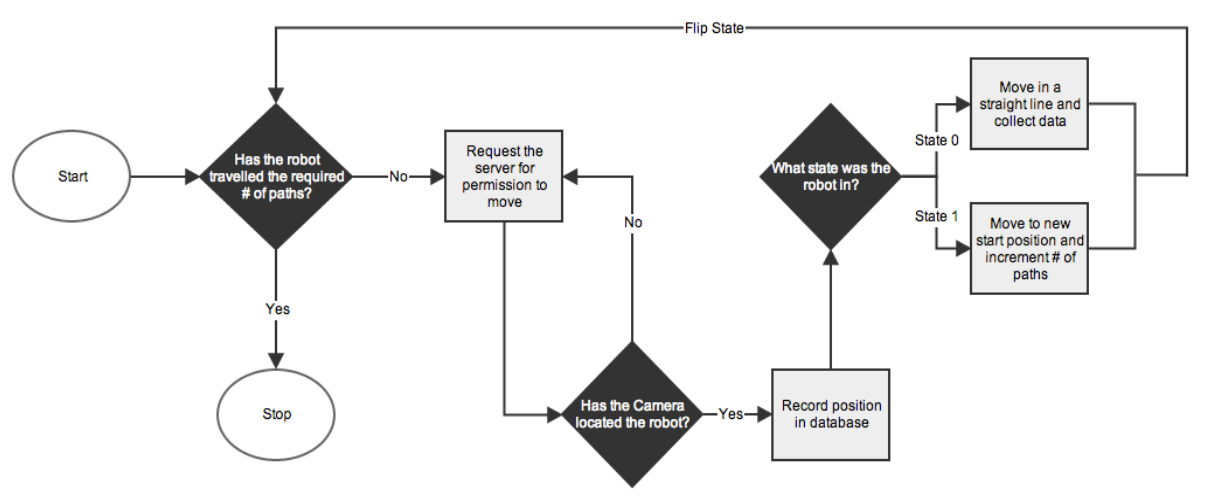
\includegraphics[width=1\linewidth]{figures/robot_flowchart}
\end{centering}

\caption{Flowchart of Robot's Logic}
\label{fig:robot-flowchart}
\end{figure}


\begin{comment}
Description of testbed, hardware, software, logic
Sid's flowchart
\end{comment}

\subsection{Noise}

Some of the factors that may affect the quality of the data collected are detailed below:
\begin{itemize}
\item \textbf{The test bed is not composed of perfectly black and white regions.} As a result, when the robot roams over what might appear to be a black region, the sensor might register a value less than the threshold and hence count it as black, or vice-versa. However, this should not cause any major issues as roaming over some distance over a white region yields sensor integral around two orders of magnitude above sensor integrals obtained by roaming over the same distance over a black region.
\item \textbf{Robot slows down with time.} The batteries wear out as the experiment goes on. So although we do not expect there to be a siginifcant difference in the speed between sucessive data points, when we consider the velocity of the robot at the first data point and its velocity at the 200th data point,there might be some difference in its velocity. The difference in velocity might be an issue as in our implementation, we integrate sensor readings over time, not distance. This would be appropriate if the velocity is constant which is a reasonable assumption for a low number of paths. But as the number of paths increases and velocity decreases, the robot would integrate fewer readings even though it travels for the same time. This will skew the data, but the seriousness of the issue has not been fully studied.
\item \textbf{Tag is not exactly centered over the sensor.} This is only a minor issue and can only be minimised to the extent that it not significant. This will not cause a constant systematic error as when the robot is travelling paths in different angles, the offset between the tag and sensor will vary. However, it is something to keep in mind and every attempt should be made to align the center of the tag with the sensor.
\end{itemize}



%%%%%%%%%%%%%%%%%%%%%%%%%%%%%%%%%%%%%%%%%%%%%%%%%%%%%%%%%%%%%%%%%%%%%%%%%%%%%%%%%%%%%%%%%%%%%%%%%%

\section{Models and assumptions}

\subsection{Problem Constraints}

Our model and lab setup were designed with the following constraints in mind: 
limited on board processing power, limited on board storage, and limited bandwidth 
(or infrequent communication with the main server). Real world examples where these constraints 
might exist include robot submarines that can only transmit data when they surface but given the massive amount of sensor information that would be collected whilst traveling in the ocean it becomes infeasible to store it all.  robot need only to sum up the the sensor readings it gets

\subsection{Mathematical Model}
Without loss of generality, we assume the area to be explored is a
rectangle denoted by $\Omega$, and the interested environment variable
$u(x,y)$ is a piece-wise constant function defined on $\Omega$.
See Figure \ref{fig:An-illustration-of-paths} for an illustration.
Assume the robot travels through $n$ different paths, which are denoted
by $C_{1},\ldots,C_{n}$. Along each path $C_{k}$, the integral of
environment variable $u$ is obtained, which is denoted by $b_{k}$.
The path integrals are written as
\begin{equation}
b_{k}=\int_{C_{k}}u(x,y)\mathrm{\,{d}\Gamma},\; k=1,\ldots,n.\label{eq:path-integral}
\end{equation}


\begin{figure}[h]
\begin{centering}

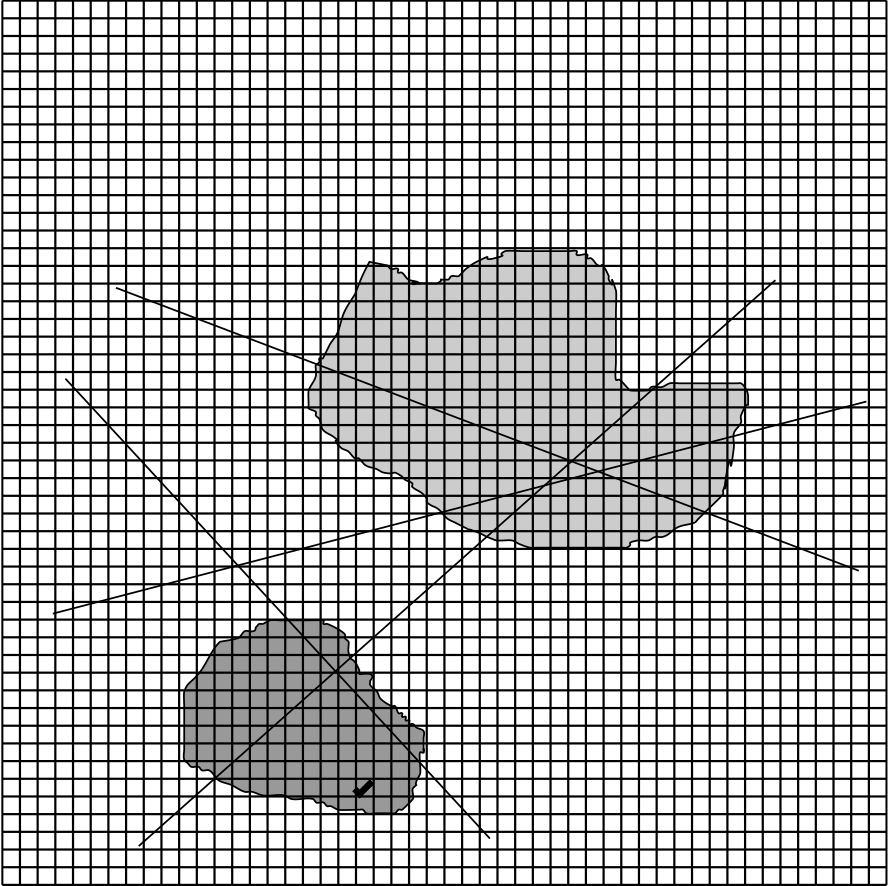
\includegraphics[width=0.5\linewidth]{figures/path-illustration}
\par\end{centering}

\caption{\label{fig:An-illustration-of-paths}An illustration of the paths
of robots. The shaded regions denote the area of interest (unknown),
where the values of environment variable $u$ is significantly different
from the surroundings. The size of the unit pixel (each small rectangle)
is determined by the accuracy of the positioning system.}
\end{figure}


For computational purpose, the whole domain is discretized into rectangular
pixels (See Figure \ref{fig:An-illustration-of-paths}). Each path
$C_{k}$ defines a weight $a_{k,ij}$ for each pixel $(i,j)$. If
$C_{k}$ does not intersect with pixel $(i,j)$, then $a_{k,ij}=0$,
otherwise $a_{k,ij}$ is defined to be proportional to the length
of the part of $C_{k}$ that falls within pixel $(i,j)$. It is also
assumed that the value of $u$ is a constant within each pixel $(i,j)$,
which is denoted by $u_{ij}$. After discretization, Eq (\ref{eq:path-integral})
becomes

\begin{equation}
b_{k}=\sum_{i}\sum_{j}a_{k,ij}u_{ij}.\label{eq:path-integral-discrete}
\end{equation}
Let $b=(b_{1},\ldots,b_{n})^{t}$, $u=(u_{ij})$, then $b$ and $u$
have a linear relation, which is written as 
\begin{equation}
Au=b,\label{eq:system-eq}
\end{equation}
where the linear operator $A$ is specified in Eq (\ref{eq:path-integral-discrete}).
Eq (\ref{eq:system-eq}) is the model equation, which poses an inverse
problem. In this equation, $b$ can be obtained from the experiment,
$A$ is determined by user-specified paths for the robot, which can
be calculated offline. $u$ is the variable that we want to solve.
Of course, if the paths form a complete raster scan over the whole
domain, then theoretically Eq (\ref{eq:system-eq}) has a unique solution.
For economical reasons, it is desirable to use much fewer paths and
still being able to reconstruct a solution for $u$. The problem is well suited for compressed sensing based image reconstruction techniques, which provide a way to solve these underdetermined systems, 

\begin{comment}
Description of constraints for our problem
limited bandwidth, data storage
Also assumptions about simple piecewise environments
\end{comment}

\section{Solving the inverse problem}

Based on the observation that the image $u$ to be reconstructed is
piecewise constant, its directional gradients, $\nabla_x u$ and $\nabla_y u$, are sparse over
the domain. We also say that there is a second operator $\Psi$, where $\Psi u$
is also sparse. For simplicity, we assume that $\Psi = I$, due to the nature 
of our experiments with the autonomous robot. That is, we can easily 
enforce the sparsity of $u$ by adjusting the size of the areas of interest with 
relation to the size of the test bed. Inspired by the compressed sensing theory, we postulate
that the actual solution $u$ should minimize the energy functional 
\[E(u) = \alpha |u|_0 + \beta\left(|\nabla_x u|_0+|\nabla_y u|_0\right),\]
where $\alpha$ and $\beta$ are parameters specifically chosen based on the nature
of $u$.

Now, let $A$ be our measurement operator as described in the previous section, and let 
$b$ be the collected samples. Then, in order to reconstruct $u$, given that we have $A$ and $b$, we must solve the optimization problem
\[ \underset{u}{{\text{{min }}}} E(u)\quad\text{such that}\; Au=b.\]
Solving this problem is intractible due to our use of the $\ell^0$ pseudo-norm, but we 
can relax it to an easily solved optimization problem by using a different sparsity-inducing 
objective function. We choose to use the $\ell^1$ norm or the nonconvex penalty function
$\varphi_p$ with $p \leq 1$, as described in the introduction. In order to account for noise 
in our data, we relax the constraint and instead use a penalty function to enforce data 
fidelity. Therefore, we can recover $u$ by solving the unconstrained optimization problem 
\begin{align}
\underset{u}{\text{min}}\text{\ }&E_{p}(u)+H(u),\label{eq:minprob}\\
\text{where }&E_{p}(u)=\alpha\varphi_p\left(u\right)+\beta\varphi_p\left(\nabla_x u + \nabla_y\right),\notag\\
&H(u)=\frac{\mu}{2}\|Au-b\|_2^2.\notag
\end{align}
Although this is a nonconvex optimization problem in the case that $p<1$,
Chartrand \cite{chartrand2009fast} and other numerical and theoretical results have shown that it can easily be solved, 
and that the solution will converge to the global minimum of the 
associated $\ell^0$ formulation. Therefore, we use the Split-Bregman method to reconstruct $u$. 

In order to use Split-Bregman, we rewrite Eq~(\ref{eq:minprob}) as
\begin{align}
\underset{u,d,d_{x},d_{y}}{{\text{{min }}}}&E_{p}(d,d_x,d_y)+H(u)\quad\text{such that}\; d=u,\, d_{x}=\nabla_{x}u,\, d_{y}=\nabla_{y}u,  \notag\\
\text{where }&E_p(d,d_x,d_y)=\alpha\varphi_p\left(d\right)+\beta\varphi_p\left(d_x +
 d_y\right).\notag
\end{align}
Then, we relax the constraints to
\begin{align*}
\underset{u,d,d_{x},d_{y}}{{\text{{min }}}}&E_{p}(d,d_x,d_y)+H(u)+B(d,d_x,d_y,u)\\
\text{where }&B(d,d_x,d_y,u)=\frac{\lambda_1}{2}\|d-u+b\|_{2}^{2}+\frac{\lambda_2}{2}\left(\|d_{x}-\nabla_{x}u+b_{x}\|_{2}^{2}+\|d_{y}-\nabla_{y}u+b_{y}\|_{2}^{2}\right),
\end{align*}
and then use our algorithm to reconstruct for $u$ through the following process described in Algorithm~\ref{split-bregman}.

\begin{algorithm}[H]
\caption{Split-Bregman method}\label{split-bregman}
\begin{algorithmic}[1]
\Procedure{Split Bregman Solve}{$A,b$}
\While{$\|u^k-u^{k-1}\|_2^2 < tol$}
\For{$n=1$ to $N$}
\State $u^{k+1}\gets \min_u{H(u)+B(d,d_x,d_y,u)}$
\State $d^{k+1}\gets \min_d{\alpha\varphi_p(d)+\frac{\lambda_1}{2}\|d-u+b\|_2^2}$
\State $d_x^{k+1}\gets \min_{d_x}{\beta\varphi_p(d_x)+\frac{\lambda_2}{2}\|d_x-\ \nabla_xu+b\|_2^2}$
\State $d_y^{k+1}\gets \min_{d_y}{\beta\varphi_p(d_y)+\frac{\lambda_2}{2}\|d_y-\ \nabla_yu+b\|_2^2}$
\EndFor
\State $b^{k+1}\gets b^{k}+\left(u^{k+1}-d^{k+1}\right)$
\State $b_x^{k+1}\gets b_x^{k}+\left(\nabla_x \left(u^{k+1}\right) - d_x^{k+1}\right)$
\State $b_y^{k+1}\gets b_y^{k}+\left(\nabla_y \left(u^{k+1}\right) - d_y^{k+1}\right)$
\EndWhile

\Return{$u\gets u^{k+1}$}
\EndProcedure
\end{algorithmic}
\end{algorithm}

This algorithm requires us to solve two different subproblems. The first problem, \[u^{k+1}=\min_u{H(u)+B(d,d_x,d_y,u)},\] has optimality condition
\[\left(\mu A^TA + \lambda_1I - \lambda_2\Delta\right)u^{k+1}=\mu A^Tb + \lambda_1(d-b)+\lambda_2\left(\nabla_x^T(d_x-b_x)+\nabla_y^T(d_y-b_y)\right),\]
so it may be solved directly. The second set of subproblems is that of computing $d^{k+1},d_x{k+1},d_y^{k+1}$. This step is easily 
accomplished by applying a generalized $p$-Shrinkage operator
\[S_\gamma^p(t)=\frac{t}{|t|}\max\left({|x|-\gamma|x|^{p-1},0}\right)\]
elementwise to $d^k,d_x^k,d_y^k$ with $\gamma = \alpha/\lambda_1, \beta/\lambda_2, \beta/\lambda_2$, respectively.

The computational bottleneck of Algorithm~\ref{split-bregman} is in fact solving for $u^{k+1}$. However, we make the assumption that 
our off-board computing power will be much greater than that of our robots. We make this claim based on the intuition that a mobile vehicle will be out collecting data for extended periods of time, during which any image reconstruction can easily be done using the data that has already been collected.

\section{Path Planning}

One of the crucial elements of our algorithm is to intelligently choose a set of paths $C=C_1,C_2,\dots,C_n$. Due to hardware 
limitations, we assume that each path is a straight-line. In order 
for accurate reconstructions to be done, it is important for the robot to explore the majority of the area to 
be mapped, $\Omega$. However, it is also important to explore less-sparse subsets of $u$ in detail, and to have a large number 
of path intersections in order to include information about specific pixels in multiple data points. We find two path planning schemes 
to be especially effective. One simply chooses $C$ randomly, and the other utilizes the data collected so far to adaptively choose the next set of samples.

\subsection{Random Paths}

The advantage of the random pathing algorithm is that it requires no off-board computation, and that we are effectively sampling in a 
random basis. Because we are sampling in a random basis, there is a high probability that our measurement basis is highly incoherent 
with the image and gradient domains. However, this is not a necessary requirement for our compressive sampling to be successful, 
because $E(u)$ is strongly convex.

Recall that each element of $C$ is a straight line. It is then simple to develop our pathing algorithm, since each path $C_k$ can be 
defined by its starting point and ending point. Let $s_k$ be the point that path $C_k$ starts at, and let $e_k$ be the end point. We generate $C$ by using Algorithm~\ref{ranpath}.

\begin{algorithm}[H]
\caption{Random path selection}\label{ranpath}
\begin{algorithmic}[1]
\Procedure{RandomPaths}{$\Omega$}
\State $s_1\gets \text{rand(}\Omega)$
\State $e_1\gets \text{rand(}\Omega)$
\For{$i=2$ to $n$}
\State $s_k\gets e_{k-1}$\Comment{Robot doesnt need to reposition.}
\State $e_k\gets \text{rand(}\Omega)$
\EndFor
\EndProcedure
\end{algorithmic}
\end{algorithm}

\subsection{Adaptive Pathing}

If off-board computing can be done, then we can process the data that has already been collected by our robot while it is collecting 
more data points. Then, it is natural to want to be able to direct the pathing process such that we are collecting data in areas that 
have high amounts of information. We propose a method of computing $C$ with such goals in mind in Algorithm~\ref{adaptivepath}. The 
algorithm is a three-step process. First, the robot collects a constant number of data points and transmits them to the server. Then, 
the server uses that data and any previously collected data to reconstruct $u$. The reconstruction, $u^*$, is then used to calculate 
a subset of points $P\subseteq\Omega$ such that each point in $P$ is a possible destination for the robot. Then, we call Algorithm~\ref{ranpath} on $P$ such that $C$ only travels to points specifically chosen based on $u^*$.

\begin{algorithm}[H]
\caption{Adaptive path selection}\label{adaptivepath}
\begin{algorithmic}[1]
\Procedure{AdaptivePaths}{$\Omega$}
\State $s_1\gets \text{rand(}\Omega)$
\State $e_1\gets \text{rand(}\Omega)$
\For{$i=2$ to $n$}
\State $s_k\gets e_{k-1}$\Comment{Robot doesnt need to reposition.}
\State $e_k\gets \text{rand(}\Omega)$
\EndFor
\EndProcedure
\end{algorithmic}
\end{algorithm}

Note that when there is no significant information about $\Omega$ collected so far, such as at the beginning of the data collection, 
we simply revert to Algorithm~\ref{ranpath} to collect the next set of data points. Also, we find in our experiments that it is 
important for there to be an element of randomness when constructing $P$. Otherwise, there is the risk that the initial set of random 
paths does not capture an important feature of $u^*$. If this is the case, then the adaptive pathing will never select those points, and will instead only produce paths where information has already been detected so far. Let us describe the method that we developed  
for choosing $P$ in more detail.


\section{Results}
\subsection{Simulated Results}

\begin{figure}[h]
\centering
\begin{subfigure}{.22\textwidth}
  \centering
    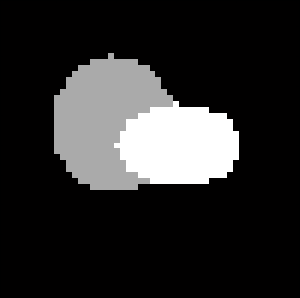
\includegraphics[width=1\linewidth]{figures/simulatedresultoriginal}
  \caption{50x50 test image.}
  \vspace{20pt}
  \label{fig:simulresorig}
\end{subfigure}%
\hspace{10pt}
\begin{subfigure}{.22\textwidth}
  \centering
    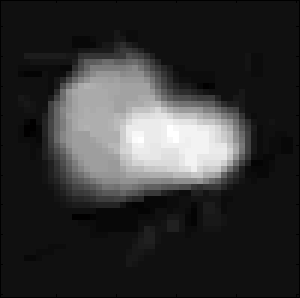
\includegraphics[width=1\linewidth]{figures/simulatedresultrec}
  \caption{Simulated reconstruction.}
  \vspace{10pt}
  \label{fig:simulresrec}
\end{subfigure}% 
\hspace{10pt}
\begin{subfigure}{.22\textwidth}
  \centering
    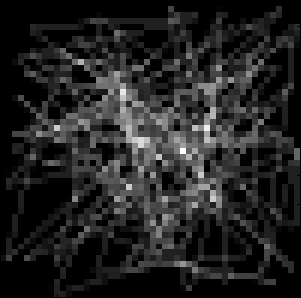
\includegraphics[width=1\linewidth]{figures/simulatedresultpaths}
  \caption{100 random paths used for simulated reconstruction.}
  \vspace{0pt}
  \label{fig:simulrespath}
\end{subfigure}%
\hspace {10pt}
\begin{subfigure}{.22\textwidth}
  \centering
    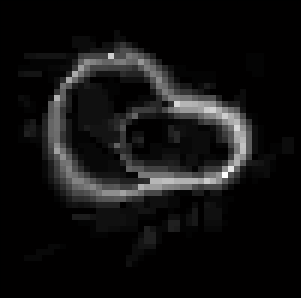
\includegraphics[width=1\linewidth]{figures/simulatedresulterror}
  \caption{Difference between the original image and the reconstruction.}
  \vspace{0pt}
  \label{fig:simulreserr}
\end{subfigure}
\caption{Simulated reconstruction using random paths.}
\label{fig:simulres}
\end{figure}

Before actually using the robot to collect data, we ran simulated reconstructions. Figure ~\ref{fig:simulresorig} is a 50x50 test image that we used for simulations. Although the lab setup required that the test bed consist of only black and white areas, in simulation, multiple shades of gray were used. Assuming the robot is capable of differentiating between the colors, the reconstruction will work just as well as it would with a black and white image.

Figure ~\ref{fig:simulresrec} is a reconstruction from 100 random paths. It is somewhat blurry, but it does reasonably well in determining the shape of the regions of interest as well as the colors of the regions. The image, being a 50x50 image, has 2500 pixels for which values must be determined. Thus, the image is being recovered from 100 data points, a 4:100 ratio of data points to values in the image.

We use Figure ~\ref{fig:simulrespath} to visualize the paths that were used in the reconstruction. For this reconstruction, the paths were generated by randomly selecting a starting point and then proceeding to randomly generate points to go to next. Thus, successive paths are connected with the end point of one path being the starting point of the next. In the figure, brighter pixels are pixels that are hit more frequently by the set of paths. Thus, this visual representation of the paths allows us to readily see what areas are more thoroughly examined and which are not.

Figure ~\ref{fig:simulreserr} shows the difference between the original image and the reconstruction. It makes it fairly clear that most of the error in the reconstruction is around the edges of the region of interest. As a means of quantifying the error, we found the norm of this difference and divided by the norm of the original image. In this particular case, this error value came to 0.2715.



\subsection{Experimental Results}

\begin{figure}[h]
\centering
\begin{subfigure}{.22\textwidth}
  \centering
    
\includegraphics[width=1\linewidth]{figures/experimentalresultoriginal}
  \caption{Image of the testbed, sized at 70x90.}
  \vspace{20pt}
  \label{fig:experresorig}
\end{subfigure}%
\hspace{10pt}
\begin{subfigure}{.22\textwidth}
  \centering
    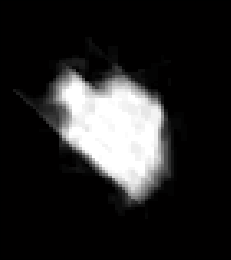
\includegraphics[width=1\linewidth]{figures/experimentalresultsimulation}
  \caption{Simulated reconstruction from the 178 paths that the robot travelled.}
  \vspace{0pt}
  \label{fig:experressim}
\end{subfigure}%
\hspace{10pt}
\begin{subfigure}{.22\textwidth}
  \centering
    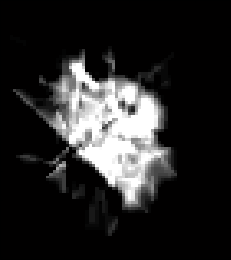
\includegraphics[width=1\linewidth]{figures/experimentalresultrec}
  \caption{Reconstruction from the data collected by the robot.}
  \vspace{10pt}
  \label{fig:experresrec}
\end{subfigure}%
\hspace {10pt}
\begin{subfigure}{.22\textwidth}
  \centering
    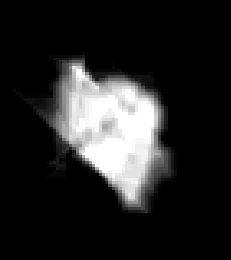
\includegraphics[width=1\linewidth]{figures/experimentalresulttunedrec}
  \caption{Reconstruction from the data collected by the robot using tuned parameters.}
  \vspace{0pt}
  \label{fig:experrestuned}
\end{subfigure}
\caption{Reconstruction using the data collected by the robot.}
\label{fig:experres}
\end{figure}

Having confirmed that our reconstruction algorithm works, we proceeded to carry out experimental testing with the actual robot. Figure ~\ref{fig:experresorig} shows a testbed that we used. The reconstruction for this testbed was carried out as a 70x90 image. As with previous simulations, the paths were generated randomly and such that the end point of one path was the starting point of the next path. This allowed the robot to gather data without having to reposition itself between paths.

As a means of comparison, we first carried out the reconstruction as a simulation, shown in Figure ~\ref{fig:experressim}. This simulated reconstruction uses the same set of 178 paths that the robot travelled along. Thus, this reconstruction is an ideal reconstruction. If the robot were able to pick up sensor values exactly as expected and with no noise, this would be the reconstruction found.

However, if we use the robot data alongside the same set of parameters as the simulated reconstruction, we instead find Figure ~\ref{fig:experresrec}. Clearly, this reconstruction is very noisy, giving black spots in the middle of the region and creating white spots where it should be black. This is due to the fact that the data collected by the robot is not as perfect as the data in simulation. As such, we retry the reconstruction, but with a lowered data fidelity parameter. This yields Figure ~\ref{fig:experrestuned}. Because there is less emphasis on fitting the image to the data, the reconstruction does a much better job. It is still not quite as accurate as the simulated reconstruction, but it is much cleaner than ~\ref{fig:experresrec} and it still does a reasonably good job of showing the region of interest.


\section{Comparison with Other Approaches}
\begin{comment}
\end{comment}

In order to judge the effectiveness of our approach, we examine other methods of collecting data and reconstructing an image. Perhaps the most intuitive manner in which to gather data about the image is to sample individual points rather than travelling and integrating along a path. As when collecting data in the form of path integrals, we would want the number of sampled points to be as low as possible. Having sampled points for data, there are then multiple approaches to recovering the image. One approach is to simply use the same Split Bregman iteration that we are using for reconstruction from path integrals, but with the individually sampled pixels. Alternatively, we can take the value found at each pixel and assign the same value to nearby pixels, a method that we refer to as pixel expansion.

\begin{figure}
\centering
\begin{subfigure}{.45\textwidth}
  \centering
    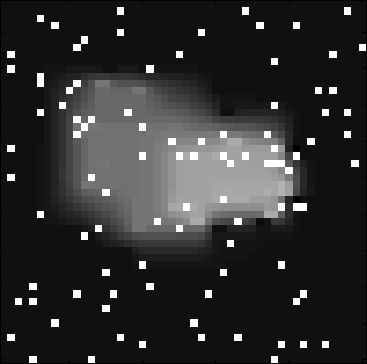
\includegraphics[width=1\linewidth]{figures/randompointreconstruction}
  \caption{Reconstruction using points sampled randomly.}
  \label{fig:randrec}
\end{subfigure}%
\hspace{10pt}
\begin{subfigure}{.45\textwidth}
  \centering
    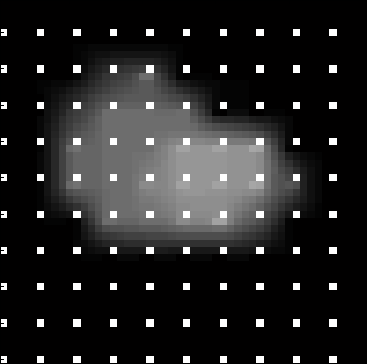
\includegraphics[width=1\linewidth]{figures/gridpointreconstruction}
  \caption{Reconstruction using points sampled on a grid.}
  \label{fig:gridrec}
\end{subfigure}
\caption{Values are found at sampled points, and Split Bregman iteration is used to reconstruct the image.}
\label{fig:samplerec}
\end{figure}

\begin{figure}
\centering
\begin{subfigure}{.45\textwidth}
  \centering
    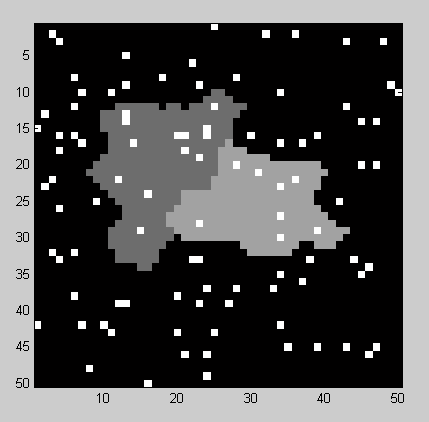
\includegraphics[width=1\linewidth]{figures/randompointexpansion}
  \caption{Expansion of points sampled randomly.}
  \label{fig:randexp}
\end{subfigure}%
\hspace{10pt}
\begin{subfigure}{.45\textwidth}
  \centering
    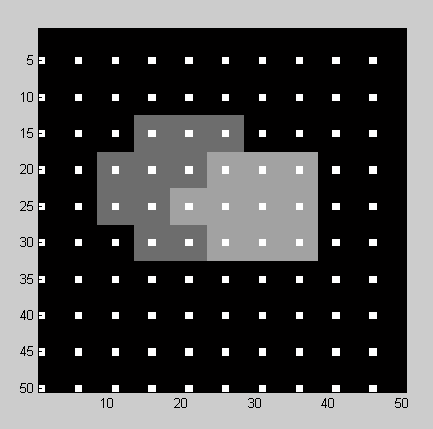
\includegraphics[width=1\linewidth]{figures/gridpointexpansion}
  \caption{Expansion of points sampled on a grid.}
  \label{fig:gridexp}
\end{subfigure}
\caption{Values are found at sampled points, and those values fill the area surrounding the sampled points.}
\label{fig:sampleexp}
\end{figure}

Figures \ref{fig:samplerec} and \ref{fig:sampleexp} present reconstructions of the previously shown 50x50 test image, Figure \ref{fig:simulresorig}, using these approaches, both with randomly sampled points and points sampled on a grid. In all cases, 100 pixels are sampled, and the sampled points are colored white.

In Figure \ref{fig:samplerec}, Split Bregman iteration was used with the collected data for reconstruction. The algorithm itself is unchanged, but the equation corresponding to a data point will simply give the value of a pixel rather than weighting pixels along the path. This method provides a moderately good reconstruction, especially in determining the general shape of the region of interest in the environment, but the demarcation between the shades of gray in the image is difficult to distinguish, making the image seem very blurry. This is not surprising because by sampling pixels, the only information gathered is about those specific pixels, so the space in between can gradate as quickly or slowly as the reconstruction algorithm deems fit. By comparing Figures \ref{fig:randrec} and \ref{fig:gridrec}, it seems that the reconstruction is more accurate when the points are sampled on a grid. This is reasonable because by sampling on a grid, the spread of sampled points is very even and well distributed. When the points are sampled randomly, certain areas will be less thoroughly investigated than others, hindering accurate reconstruction.

Figure \ref{fig:sampleexp} illustrates pixel expansion. This is done by looping through every pixel in the image, and for each pixel, finding and assigning the value from the nearest pixel that was sampled. This process creates expanded pixels of a single color around each sampled pixel. When the pixels are sampled on a grid, the even distribution causes the expanded pixels to simply be squares, essentially creating a low resolution version of the image, as in Figure \ref{fig:gridexp}. Figure \ref{fig:randexp} is a result of pixel expansion with randomly sampled pixels. The unpredictable spread of sampled pixels causes the expanded pixels to vary widely in shape and size, and the reconstruction does a poor job of determining the shape of the region of interest.

To compare these methods, Figure \ref{fig:othermethoderror} plots the error of these approaches, as well as the path integral reconstruction that we are actually carrying out, with respect to the number of data points collected. The blue line represents reconstruction from randomly generated path integrals, and as desired, for a low number of data points, it has lower error than the other methods. As the number of samples grows, all methods begin to have similar error; this is expected because any method will work reasonably well with enough data. Worth noting is that while pixel expansion from samples on a grid appears to do better than random path integrals for some of the low data situations, the effectiveness of grid point expansion is highly variable, and as such, its overall usefulness is limited. The accuracy of reconstruction is very dependent on how well the grid aligns with the given image, and choosing the best grid size for a given environment would require prior knowledge of the environment. Another flaw with pixel expansion is the dependence on accurate sampling; pixel expansion will be very heavily affected by noise. If a pixel is sampled inaccurately, the entire expanded pixel associated with that sample will be inaccurately reconstructed. Using Split Bregman iteration mitigates this issue, and using path integrals further diminishes the impact that a single inaccurate sample can have.


\section{Adaptive Pathing}
\begin{comment}
\end{comment}

\subsection{Simulated Results}
\begin{figure}
\centering
\begin{subfigure}{.22\textwidth}
  \centering
    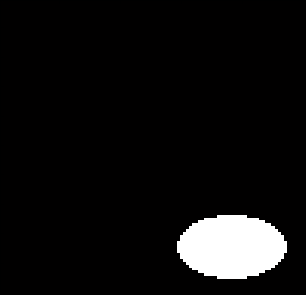
\includegraphics[width=1\linewidth]{figures/adaptiveresultoriginal}
  \caption{100 x 100 pixel test image with the area of interest in bottom right corner.}
  \vspace{0pt}
  \label{fig:adp_sim_orig}
\end{subfigure}%
\hspace{10pt}
\begin{subfigure}{.22\textwidth}
  \centering
    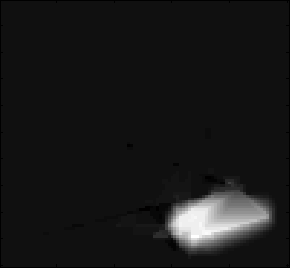
\includegraphics[width=1\linewidth]{figures/nonadaptiveresultrec}
  \caption{Simulated reconstruction from the 200 paths}
  \vspace{0pt}
  \label{fig:adp_randpaths_sim_rec}
\end{subfigure}%
\hspace{10pt}
\begin{subfigure}{.22\textwidth}
  \centering
    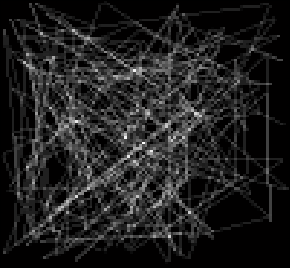
\includegraphics[width=1\linewidth]{figures/nonadaptiveresultpath}
  \caption{The 200 randomly generated paths.}
  \vspace{0pt}
  \label{fig:adp_randpaths_sim}
\end{subfigure}%
\hspace {10pt}
\begin{subfigure}{.22\textwidth}
  \centering
    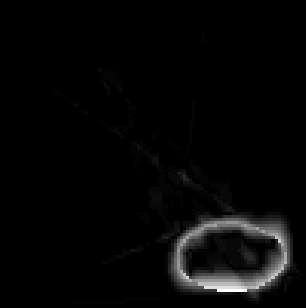
\includegraphics[width=1\linewidth]{figures/nonadaptiveresulterror}
  \caption{Difference between the original image and the reconstruction}
  \vspace{0pt}
  \label{fig:adp_randpaths_diff}
\end{subfigure}%
\caption{Simulated reconstruction using random paths as before.}
\label{fig:adp_randpaths_fig}
\begin{subfigure}{.22\textwidth}
  \centering
    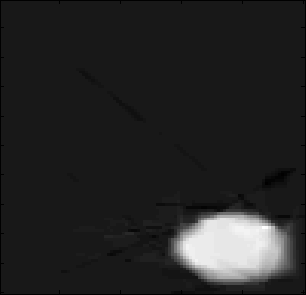
\includegraphics[width=1\linewidth]{figures/adaptiveresultrec}
  \caption{Simulated reconstruction from 200 adaptive paths.}
  \vspace{0pt}
  \label{fig:adp_adpaths_sim_rec}
\end{subfigure}%
\hspace{10pt}
\begin{subfigure}{.22\textwidth}
  \centering
    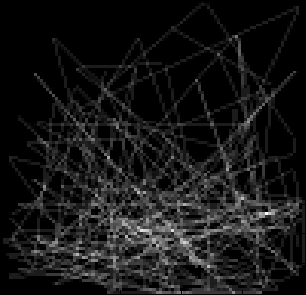
\includegraphics[width=1\linewidth]{figures/adaptiveresultpath}
  \caption{The 200 adaptive paths.}
  \vspace{0pt}
  \label{fig:adp_adpaths}
\end{subfigure}%
\hspace {10pt}
\begin{subfigure}{.22\textwidth}
  \centering
    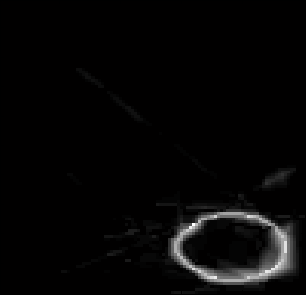
\includegraphics[width=1\linewidth]{figures/adaptiveresulterror}
  \caption{The difference between the reconstruction and original image.}
  \vspace{0pt}
  \label{fig:adp_adpaths_sim_diff}
\end{subfigure}
\caption{Reconstruction using the adaptive paths.}
\label{fig:adp_adpaths_sim_fig}

\end{figure}
As with the previous reconstruction method, we first ran simulations on a test image to see if this method would provide better results. Figure \ref{fig:adp_sim_orig} is a 100x100 binary image with a white, ellipse shaped area of interest in the bottom right corner that was used as a test image. As a control we first run the simulation with the same algorithm as before to test against the new adaptive pathing algorithm. The expectation is that with the same number of paths the adaptive pathing algorithm yields a lower error (alternatively we could also test to see if we could get the same error with fewer paths).  

Figure \ref{fig:adp_randpaths_sim} shows the 200 random paths taken by the simulation. As before, these are simulated robot paths so the end point of one path is the starting point for the subsequent path. The brightness of each pixel corresponds to how often (and with how much weighting) a path traveled through that area. 

The reconstruction obtained with these paths is shown in Figure \ref{fig:adp_adpaths_sim_rec}. This reconstruction is able to recover successfully generally the region of interest and the size of the area, but is not able to ascertain some of the more detailed information about the shape and boundary of the area accurately. 

Figure \ref{fig:adp_randpaths_diff} shows the difference between the the reconstructed image and the ground truth. The error is primarly along the edges but more prominent along the bottom edge. The norm of the difference divided by the norm of the original is <INSERT VALUE HERE>.

We compare these results against those displayed in Figure \ref{fig:adp_adpaths_sim_fig}, which are generated by the adaptive pathing algorithm on the same test image in \ref{fig:adp_sim_orig}. 

Figure \ref{fig:adp_adpaths} shows the 200 adaptive paths taken by the simulation. There are visibly clustered near the bottom of the image, where it identified early on had the area of interest. Figure \ref{fig:adp_adpaths_sim_rec} then shows the results of the Split Bregman reconstruction with the data collected from the adaptive paths. Because the paths examined the area more closely, the reconstruction is able to more accurately capture the curve along the borders and thus the shape of the area itself. This is illustrated in Figure \ref{fig:adp_adpaths_sim_diff}, which shows the difference between this reconstruction and the original test image. The norm of the difference divided by the norm of the original is <INSERT VALUE HERE>, which is significantly lower than the reconstruction done by purely random paths.

\subsection{Experimental Results}

\begin{figure}
\centering
\begin{subfigure}{.4\textwidth}
  \centering
    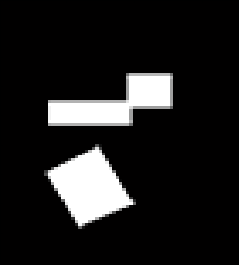
\includegraphics[width=1\linewidth]{figures/adaptiveexperimentalresultoriginal}
  \caption{Image of the testbed, sized at 70x90}
  \vspace{0pt}
  \label{fig:adp_exp_orig}
\end{subfigure}%
\hspace{10pt}
\begin{subfigure}{.4\textwidth}
  \centering
    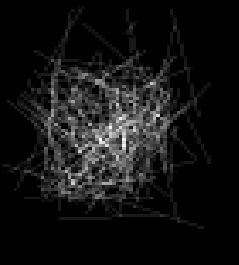
\includegraphics[width=1\linewidth]{figures/adaptiveexperimentalresultpath}
  \caption{The 224 adaptive paths traveled by the robot}
  \vspace{0pt}
  \label{fig:adp_exp_paths}
\end{subfigure}%
\hspace{10pt}
\begin{subfigure}{.3\textwidth}
  \centering
    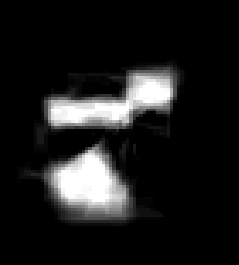
\includegraphics[width=1\linewidth]{figures/adaptiveexperimentalresultsimulation}
  \caption{Simulated reconstruction for the adaptive paths traveled by the robot}
  \vspace{0pt}
  \label{fig:adp_exp_recon_simmed}
\end{subfigure}%
\hspace{10pt}
\begin{subfigure}{.3\textwidth}
  \centering
    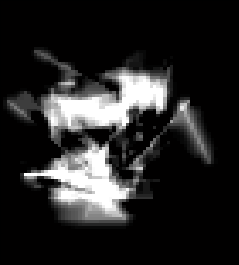
\includegraphics[width=1\linewidth]{figures/adaptiveexperimentalresultrec}
  \caption{Image reconstruction using robot collected data}
  \vspace{0pt}
  \label{fig:adp_exp_recon_untuned}
\end{subfigure}%
\hspace {10pt}
\begin{subfigure}{.3\textwidth}
  \centering
    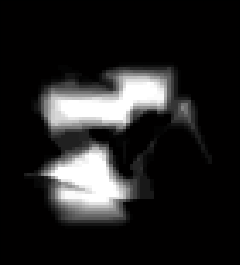
\includegraphics[width=1\linewidth]{figures/adaptiveexperimentalresulttunedrec}
  \caption{Image reconstruction using robot collected data with tuned parameters}
  \vspace{0pt}
  \label{fig:adp_exp_recon_tuned}
\end{subfigure}
\caption{Experimental results of adaptive pathing using robot collected data}
\label{fig:adp_exp_fig}
\end{figure}
Once we were able to confirm that adaptive pathing could yield better results, we implemented it in the lab with our robot vehicle and the results are shown in Figure \ref{fig:adp_exp_fig}. Figure \ref{fig:adp_exp_orig} is an image of the original testbed, sized to 70x90, which contains multiple areas of interest that are off center and have sharply defined edges, which tests the adaptive pathing algorithm's ability to distinguish between objects, find areas of interest, and reconstruct them with some detail. 

Figure \ref{fig:adp_adpaths} shows the 224 straight line paths the robot vehicle traveled on the testbed and it can be observed that it did not travel often to black areas or corners where there were no areas of interest.

We then generate Figure \ref{fig:adp_exp_recon_simmed}, which is an ideal reconstruction (how the simulation would run if data could be collected with no noise). If we run the same reconstruction with robot data, the resulting reconstruction is significantly affected by the noise in the data, as shown in Figure \ref{fig:adp_exp_recon_untuned}. Because of the sources of noise described earlier, such as the testbed not being entirely black and the sensor sometimes taking incorrect readings, the resulting reconstruction appears to have streaks of areas that do not exist in the original image. To account for noise in the data, we again tune the parameters in our minimization problem and lower the data fidelity term. With greater importance placed on minimizing the gradient, we obtain \ref{fig:adp_exp_recon_tuned}, which is a more accurate reconstruction and is much closer to reconstruction that assumes no noise.
\section{Conclusions and Further Work}

\newpage
\bibliographystyle{plain}
\bibliography{resources.bib}


\newpage
\section{Appendix}

\subsection{README.txt for Data Collection}

\begin{verbatim}

FILE: README.txt
AUTHOR: Siddarth Srinivasan (UCLA REU 2014)
DATE: 11th August 2014


Contents
--------

I.    Introduction
II.   Applications Needed to Run this Project
III.  Libraries
IV.   Drivers
V.    Code Documentation
VI.   Arduino Pins
VII.  Hardware on Robot
VIII. Other Hardware
IX.   Setup
X.    Run
XI.   Other Issues
XII.  Future Improvements


I. Introduction
---------------
This file details all the applications, libraries and drivers needed to ensure
the project runs smoothly, and provides instructions to set up and run the
project. Full code documentation can be found at:
		C:\REU\2014\Server\Documentation\html\index.html
"The project" refers to the "Environental Mapping by Autonomous Robots Using
Compressed Sensing" project completed by the UCLA Computational and Applied Math
REU 2014 Team consisting of M. Horning, S. Zou, S. Srinivasan and M. Lin.

At the time of writing, all project files are in C:\REU_Server_2014 on
MUFASA-PC. See setup-server below on what is affected when changes are made.


II. Applications Needed to Run this Project
-------------------------------------------
1) XAMPP: to set up Apache server and MySQL database
2) Arduino IDE: to upload programs to the robot and view output on Terminal
3) Python 2.7: to run vehicle\_tracker.py and the server cgi script
4) MATLAB: to carry out the image reconstruction


III. Libraries
--------------
1) Arduino Libraries:
	*   AdaFruit WiFi Shield Library: to enable the arduino to connect to
	  wireless networks.
	*   Arduino Json Library: so that the Arduino can parse the response from
	  the server.

2) Python Libraries:
	*   OpenCV: to use the camera to track the robot on the testbed.
	*   PySerial: to read and write Serial Data to COM ports
	*   MySQL connector: to enable python to perform SQL commands with databases
	*   PythonWin: to enable python to commmunicate with MATLAB


IV. Drivers
-----------
1) Prolific 2303 Serial Driver: To recognize the USB-Serial cable
	http://www.prolific.com.tw/US/ShowProduct.aspx?p_id=229&pcid=4
2) Generic 1394 Camera Driver: To recognize the overhead cameras on Firewire
	http://www.driverscape.com/download/generic-1394-desktop-camera


V. Code Documentation
---------------------
1) Accessing Documentation/html/index.html should show you the doxygen generated
  documentation for the project. THE CGI SCRIPTS HAD TO HAVE THEIR EXTENSIONS
  CHANGED TO .PY BEFORE DOXYGEN COULD BE RUN, SO KEEP THAT IN MIND. 
2) Doxywizard can be run from cmd to configure the doxygen output, or edit and
 run doxygen doxygen from C:\REU_2014_Server.
3) The .cgi and .py scripts are documented under "Packages" and the .ino file is
  documented under "Files"


VI. Arduino Pins
----------------
1) The pins used by the WiFi Shield can be found at:
	https://learn.adafruit.com/adafruit-cc3000-wifi/connections
2) Digital Pins 6-9 are used to control the motor.
3) Analog Pin 4 is connected to the reflectance sensor.


VII. Hardware on Robot
----------------------
1) Arduino Uno
		http://arduino.cc/en/Main/arduinoBoardUno
   with AdaFruit WiFi Shield
   		http://www.adafruit.com/products/1491

2) NEOMART L298N Motor Controller:
		https://s3.amazonaws.com/tontec/l298n.zip

3) DFRobot 4WD Chassis with 4 motors:
  		http://www.amazon.com/DFRobot-Pirate-4wd-Mobile-Platform/dp/B009646R3K/ref=sr_1_cc_2?s=aps&ie=UTF8&qid=1408062128&sr=1-2-catcorr&keywords=dfrobot+4wd

4) Rectangular white tag with black boundary and black header strip

5) 5x 1.5V AA Battery to power motors
		http://www.amazon.com/AmazonBasics-Precharged-Rechargeable-Batteries-16-Pack/dp/B007B9NV8Q/ref=sr_1_2?ie=UTF8&qid=1408062203&sr=8-2&keywords=amazon+batteries+aa

6) 9V EBL battery to power Arduino
		http://www.amazon.com/EBL%C2%AE-Battery-Charger-Rechargeable-Batteries/dp/B00HV4KFSA/ref=sr_1_1?ie=UTF8&qid=1408062243&sr=8-1&keywords=9v+rechargeable+ebl


VIII. Other Hardware
--------------------
1) USB to Serial Cable (Use Prolific 2303 Driver):
		http://www.adafruit.com/blog/wp-content/uploads/2011/01/usbserial_MED.jpg

2) Serial Cable:
		http://www.homanndesigns.com/store/images/DB9F-DB9M_Serial_cable.jpg

3) Two Wi232 Transceivers: Download configuration tool from here
		http://mikrokopter.de/ucwiki/RadioTronix#Download_Konfigurationstool
   It has currently been installed on this computer. It is used to test the 
   Wi232 transceivers, and set the channel on which the transmit and receive. To
   configure (it should already be configured, so you wouldn't normally need to
   do this):

   		a) Switch the jumper on the Wi232 while the transceiver is still on.
   			When the jumper is on the two pins towards the red LED and away from
   			the switch, it is in "USE" mode.
   			When the jumper is on the two pins close to the switch and away from
   			the LED, it is in "DEBUG" mode.
   			IMPORTANT: DO NOT SWITCH OFF AND SWITCH ON THE TRANSCEIVER WHEN THE
   			JUMPER IS IN THIS "DEBUG" MODE, IT WILL RESET THE CHANNELS TO
   			DEFAULT.
   		b) Open "Radiotronix Wi.232DTS Evaluation", select the COM port and the
   		   Baud Rate (should be 115200) and click on "Discover module".
   		c) Click on "Read" on the Transmit Channel and Receive Channel, and note
   		   down the channel.
   		d) Move the jumper back to "USE" mode.
   		e) Do the same thing with the other transceiver, and check that the
   		   transmission channel of each transceiver matches the receiving
   		   channel of the other transceiver.

4) TP-LINK Router: Used to broadcast the private network on which the server
				   will be hosted. To configure, connect to the computer by
				   ethernet and go to 192.168.0.1 and enter user: admin and
				   password: admin.


IX. Setup
---------
1) Cameras:
	*   Ensure that the two cameras are plugged into the FireWire ports.
	*   Check Device Manager -> Imaging Devices to make sure the drivers are
	  installed and working properly.
	*   Ensure that the USB-Serial cable is plugged in and connected to the
	  Wi232 transceiver, and the COM_PORT in vehicle_tracker.py matches the COM
	  port that shows up in Device Manager. This is the COM port that the
	  overhead camera will write to.
	*   Also ensure that the transceiver is powered on.
	*   You should be able to run vehicle_tracker.py.
	*   vehicle_tracker.py will quit and restart every so often. (Refer to 
	  known issues).
	*	ONLY QUIT vehicle_tracker.py by pressing 'q'. Otherwise, you may get an
		error (see Known Issues) the next time you try to run it.

2) Server:
	*   Launch XAMPP and start Apache and MySQL.
	*   Check that in the file Apache -> Config -> httpd.conf (as accessed from
	  XAMPP), the DocumentRoot and Directory in Line 242-243 are set to the
	  folder containing the server files. At the time of writing, it is set to
	  "C:\REU_2014_Server". If this is changed, the Arduino will also have to
	  change its request (see Robot).
	*   The server files are robotServer.cgi and databaseManager.cgi. Both can
	  be accessed at C:\REU_2014_Server\.
	*   Login to localhost/phpmyadmin with user: root and password: uclaRobots14
	  to access the databases.
	*   Goto localhost/databaseManager.cgi to create, clear or delete databases.
	*   Ensure that the serial cable is connected to the Wi232 transceiver, and
	  the transceiver is powered on.
	*   Also ensure that the COM_PORT in robotServer.cgi matches the COM port
	  that shows up in Device Manager. This is the COM port to read robot's
	  position from.
	*   Check that dbName in robotServer.cgi matches the name of the database
	  you wish to access.
	*   Test localhost/robotServer.cgi by entering states 0 or 1 (other states
	  will not work, and state 1 requires data submission) and checking the
	  database at localhost/phpmyadmin for changes in State_Record.
	*   You will want to clear the database after testing.
	*   'State_Record' keeps track of all communications with the server,
		'Data_Collection' is the final data table and 'Next_Paths' is the SQL
		table storing the next set of paths.

3) Robot:
	*   Launch Arduino IDE, connect the Arduino to the computer and check that
	  it has been detected on Tools -> Serial Port.
	*   Use and modify motor_ir_test.ino in Miscellaneous to calibrate
	  PIXELS_PER_SECOND and RADS_PER_SECOND. Run vehicle_tracker.py and observe
	  change in x or y as the robot moves vertically or horizontally for 1
	  second for PIXELS_PER_SECOND and change in theta as the robot rotates for
	  1 second for RADS_PER_SECOND.
	*   Use ir_test.ino to verify MAX_SENSOR and WHITE_BOUNDARY by placing the
	  reflectance sensor of black and white regions on the test bed.
	*   The file for robot logic is compressedSensing.ino.
	*	Check that the WLAN_SSID, WLAN_PASS, WLAN_SECURITY, IP, Port and 
	  repository in compressedSensiong.ino match the network you wish to use.
	  ipconfig on cmd will give you the ip-address of the network the server is
	  on.
	*   Ensure the chassis is covered with black tape, so that the camera
	  doesn't confuse some part of the chassis for the tag.
	*   Set NUM_PATHS in compressedSensing.ino to 1 more than the number of
	  paths you want the robot to travel.
	*   Upload compressedSensing.ino to the Arduino.


X. Run
------
1) Launch vehicle_tracker.py.
2) Launch XAMPP and start Apache and MySQL.
3) Place the Arduino on the test bed and connect the board to the battery.
4) Once the data has been collected in MySQL, export it to a csv and put it
   in the same folder as reconstructImage.m MATLAB script. Edit that file
   to ensure that the file it's pulling data from is the file you have just
   downloaded, and run the file.


XI. Known Issues
----------------
1) Off the test bed: Occasionally, the video camera might make a mistake and
  					 accidentally send the robot off the test bed. If that
  					 happens, put the robot back on the test bed and ignore
  					 that data point.
2) Select Video Source: If vehicle_tracker.py is not quit properly, the next
						time it is run, it may ask you to select a video source,
						but still give you trouble. To solve this, open Task
						Manager and end pythonw.exe that takes around 30,000 K.
						If this still doesn't work, end all the pythonw.exe
						processes and run vehicle_tracker.py again.
3) Cannot open a camera: Unplug and replug in the firewire connections. Also
						 check the Device Manager. For some reason, checking
						 Device Manager makes it work again. 
4) Shifting image: The video displayed by vehicle_tracker.py unpredictably gets
 				   shifted sometimes. Unknown reason, but if that happens,
 				   restart vehicle_tracker.py. Current fix includes restarting
 				   the camera every RESET number of iterations.
5) Parallax: The tag is not exactly centered at the reflectance sensor, and may
			 cause some noise in the data.
6) MATLAB: Currently, MATLAB is having issues plotting images, so the actual
		   image reconstruction is carried out on another computer. The
		   adaptive path selection using MATLAB still works without problems.
		   So to recontruct data,


XII. Future Improvements
------------------------
1) Eliminate the need for the Wi232 transceivers by creating virtual ports or
  sockets, so that the server-side script can communicate with
  vehicle_tracker.py without external hardware.
2) Write small test programs for the individual libraries.
3) Extend the analog sensor for use with images with varying shades of grey.
  Currently, a reading from the reflectance sensor is characterised as black or
  white based on the reading. Add more 'buckets' based on the range of values.
4) Write a script that can access the 'State_Record' and display the current
  status of the robot. This will save time from trying to make sense of the
  status data in 'State_Record'.
\end{verbatim}



\subsection{Code Documentation (refman.pdf)}

\end{document}
